\documentclass[25pt]{article}
    \usepackage[a4paper, top=3cm, left=3cm, right=2.5cm, bottom=2.5cm]{geometry}
    \usepackage{lmodern}
    \usepackage[T1]{fontenc}
    \usepackage[portuges]{babel}
    \usepackage[utf8]{inputenc}
    \usepackage{a4}
    \usepackage[document]{ragged2e}
    \usepackage{textgreek}
    \usepackage{epstopdf}
    \usepackage{graphicx}
    \usepackage{fancyvrb}
    \usepackage{amsmath}
    \usepackage{float}
    \usepackage{listings}
    
    
    \begin{document}
    
    \begin{titlepage}
    
    \newcommand{\HRule}{\rule{\linewidth}{0.5mm}} % Defines a new command for the horizontal lines, change thickness here
    
    \center % Center everything on the page
    
    %----------------------------------------------------------------------------------------
    %	HEADING SECTIONS
    %----------------------------------------------------------------------------------------
    
    \textsc{\LARGE Universidade do Minho}\\[1.5cm]
    \HRule \\[0.4cm]
    { \huge \bfseries Processador Flex}\\[0.4cm]
    \HRule \\[1.5cm]
    \textsc{\Large Mestrado Integrado em Engenharia Informática}\\[0.5cm]
    \textsc{\large Processamento de Linguagens}\\[0.5cm]
    \textsc{\large 2ºSemestre 2018/19}\\[0.5cm]
    
    
    %----------------------------------------------------------------------------------------
    %	AUTHOR SECTION
    %----------------------------------------------------------------------------------------
    
    \begin{minipage}{0.4\textwidth}
    \begin{flushleft} \large
    \emph{Grupo:}\\
    Joana Cruz A76270 \\
    Rui Azevedo A80789 \\
    Maurício Salgado A71407 \\
    \end{flushleft}
    \end{minipage}
    ~
    \begin{minipage}{0.4\textwidth}
    \begin{flushright} \large
    \emph{Docentes:} \\
    Pedro Rangel Henriques\\
    José João Almeida\\
    \end{flushright}
    \end{minipage}\\[2cm]
    
    %----------------------------------------------------------------------------------------
    %	DATE SECTION
    %----------------------------------------------------------------------------------------
    
    {\large \today}\\[2cm]
    
    %----------------------------------------------------------------------------------------
    %	LOGO SECTION
    %----------------------------------------------------------------------------------------
    
    % \includegraphics[scale=0.3]{uminho}\\
    
    %----------------------------------------------------------------------------------------
    
    \vfill % Fill the rest of the page with whitespace
    
    \end{titlepage}
    \section{Resumo}
    O presente trabalho tem como objetivo aumentar a experiência no uso do ambiente Linux, aumentar capacidade de escrever 
    Expressões Regulares (ER) e, a partir destas, desenvolver Processadores de Linguagens Regulares.
    A ferramenta de processamento de texto utilizada é o C Flex que, por sua vez, também utiliza o GCC.
    
    \newpage
    \tableofcontents
    \newpage
    \section{Introdução}
    \subsection{Preliminares}
    A diversidade e quantidade de informação atualmente é cada vez maior e mais dispersa.
    Assim, torna-se ainda mais necessária uma linguagem de programação como o 
    C Flex, que permite filtrar, de maneira facilitada, a informação essencial num ficheiro em que os dados estejam dispersos 
    e ainda tratar essa informação. O trabalho apresentado na unidade curricular de Processamento de Linguagens tem como 
    objetivo usar esta ferramenta para filtrar um conjunto de dados fornecidos, extraindo desses dados informação relevante.
    \subsection{Sele\c{c}\~ao de enunciado e Objetivos}
    De seguida, apresentamos o tema proposto ao grupo, sendo este o Jornal Angolano versão 2. \\

    Dado um ficheiro com alguns milhares de notícias do jornal angolano "Folha 8",
    pretendemos:
    \begin{enumerate}
    \item Limpar e normalizar os artigos.
    \item Criar HTML correspondente:
      \begin{itemize}
        \item criar um ficheiro HTML (post-6243.html)  por cada notícia.
        \item juntar um link para o ficheiro com texto "título" em cada índice de "tag"
      \end{itemize}
    
    \item Criar uma lista das tag encontradas e respectivos números de ocorrências.
    \end{enumerate}
    \subsection{Estrutura do Relatório}
    Inicialmente vai ser explicado o problema, as características dos dados fornecidos e os padrões de frase
    encontrados e que levaram à resolução do trabalho proposto.
    Numa segunda fase apresentamos a codificação em Flex da solução desenvolvida mostrando as estruturas de dados e
    ações semânticas, bem como alternativas e decisões tomadas face aos problemas de implementação.
    Por último mostramos exemplo de um input e output e, também, em apêndice a este relatório está também todo o código desenvolvido.
    \subsection{Características dos Dados, Padr\~oes de Frase e Decisões}
    O programa a desenvolver tem por propósito receber um ficheiro com alguns milhares de notícias, e primeiramente limpar e normalizar
    esses artigos. Para isso é necessário encontrar certos padrões para conserguirmos extrair a informação útil.
    A informação que consideramos fundamental extrair de cada notícia foi: as tags, o identificador, a
    categoria do jornal, o título, a data da redação, e por último o texto da notícia. Consideramos tudo o resto como informação não relevante. 
    Com esta informaçao recolhida conseguimos gerar o HTML correspondente à noticia. Entretanto, durante a filtragem vamos armazenando 
    numa estrutura de dados informação necessária de modo a cumprir os outros objetivos do trabalho, que será explicado posteriormente.
    \newpage
    \section{Implementação e Ações Semânticas}
    Após uma análise detalhada de diversas notícias do Jornal Angolano, conseguimos identificar certos padrões, e definir certos estados que nos
    ajudariam no processamento correto do ficheiro. 
    \subsection{Estados e Expressões Regulares}
    Definimos as seguintes start conditions:
    \begin{verbatim}
    %x TAGS
    %x TAG
    %x DATE
    %x ID
    %x CLEAN
    %x CATEGORY
    %x TITLE
    %x TEXT
    \end{verbatim}
    Inicialmente cada notícia apresenta as tags, o estado é alterado de INITIAL para TAGS sempre que encontra a expressão \#TAG:
    Dentro deste estado sempre que o texto corresponder com a expressão tag:\{, o estado é alterado de TAGS para TAG.
    Também definimos que quando corresponder com um novo \# sabemos que encontramos todas as tags, não podia ser uma quebra de linha
    devido a algumas tags se encontrarem em diferentes linhas, e regressamos ao estado INITIAL.
    \begin{verbatim}
        #TAG:   		        {BEGIN TAGS; numberTags = 0;}
        <TAGS>tag:\{     {BEGIN TAG;}
        <TAGS># 		        {BEGIN INITIAL;}
    \end{verbatim}
    Neste estado guardamos a informação relativa à tag, e sempre que encontra o final de uma tag identificado por uma \}, retorna
    ao estado anterior.
    \begin{verbatim}
        <TAG>\}   	    {BEGIN TAGS;}
        <TAG>[^}]+ 		   {tagsPost[numberTags++]=strdup(yytext);}
    \end{verbatim}
    Em cada notícia, sempre que encontramos a expressão ID:\{ o estado é alterado de INITIAL para ID, e apenas nos interessa o identificador do post, 
    logo apenas guardamos a informação até encontramos um espaço. De seguida, entramos para o estado CLEAN. Este encadeamanento
    de estados foi necessário, pois de seguida encontraremos a categoria e o título que não tem nenhuma expressão para os identificar.
    \begin{verbatim}
        ID:\{			        {BEGIN ID;}
        <ID>[^ ]+		    {id = strdup(yytext); BEGIN CLEAN;}
    \end{verbatim}
    Processamos tudo até encontrar uma \} seguida de uma quebra de linha, e alteramos para o estado CATEGORY.
    \begin{verbatim}
        <CLEAN>[^}]+\}\n	    {BEGIN CATEGORY;}
    \end{verbatim}
    Na categoria, interessa-nos processar tudo o que se encontra nessa linha, e guardar numa variável. Encontramos o padrão que após duas quebras de linha começa sempre o título.
    \begin{verbatim}
        <CATEGORY>.+\n\n    {yytext[yyleng-2] = '\0'; 
                            category = strdup(yytext); 
                            BEGIN TITLE;}
    \end{verbatim}
    Quando entramos no estado TITLE processamos tudo o que se encontra na linha, e finalmente regressamos ao estado INITIAL.
    \begin{verbatim}
        <TITLE>.+		        {title = strdup(yytext);}
        <TITLE>\n\n       {BEGIN INITIAL;}
    \end{verbatim}
    Em cada notícia, sempre que encontramos a expressão \#DATE: , seguido de [ com um conjunto de caracteres possíveis como letras e algarismos(que não nos interessa filtrar)
    seguido de possíveis espaços, entramos no modo DATE. Após isso, filtramos tudo até uma quebra de linha, guardando numa variável a data. De seguida sabemos que o padrão
    é uma quebra de linha, seguido de qualquer caracter(pode aparecer normalmente o título outra vez, ou simplesmente texto que não nos interessa processar), 
    e de seguida após duas quebras de linha encontra-se o texto correspondente da notícia.
    \begin{verbatim}
        #DATE:\ *\[[^]]+\]\ *   {BEGIN DATE;}
        <DATE>[^\n]+ 		 	        {date = strdup(yytext);}
        <DATE>\n[^\n]*\n\n 		    {BEGIN TEXT;}
    \end{verbatim}
    Neste último modo por nós definido, processamos todo o texto até encontrarmos o símbolo < que nos indica que chegamos ao fim da notícia.
    \begin{verbatim}
        <TEXT>[^<]+	    {text = strdup(yytext); BEGIN INITIAL;}
    \end{verbatim}
    Sabemos sempre que uma notícia acaba quando encontramos a expressão </pub>, pelo que aqui iremos criar o HTML corresponde à notícia com a informação guardada previamente.
    \begin{verbatim}
        \<\/pub\>	       {FILE *fp;
                        char * idPost = strdup(id);
                        char *idP = strcat(idPost,".html");
                        fp = fopen(idP, "w");
                        fprintf(fp, "<html>\n<head>\n\t<meta charset=\"UTF-8\">\n\t
                        <pub id =%s>\n\t<title>%s</title>\n</head>\n", id, title);
                        fprintf(fp, "<body>\n\t<h2><author_date>%s</author_date></h2>\n
                        \t<hr>\n\t<p>\n\t<tags>Tags:\n", date);
                        for(j= 0; j < numberTags; j++){
                            generate(tagsPost[j], title, idP, ltag);
                            fprintf(fp,"\t\t<li><tag>%s</tag></li>\n", tagsPost[j]);
                        }
                        fprintf(fp,"\t</tags>\n\t</p>\n\t<hr>\n\t<p>\t<category>%s</category></p>\n
                        \t<hr>\n\t<text>\n%s\n\t</text>\n</body>\n</html>", category, text);
                        fclose(fp);}
    \end{verbatim}
    \begin{figure}
    \centering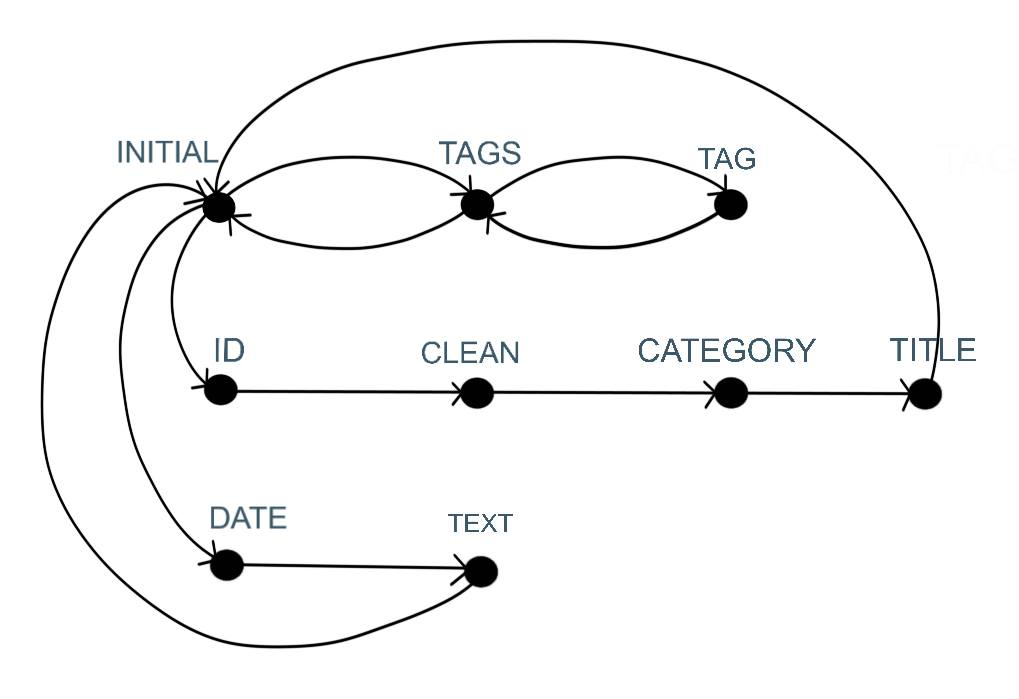
\includegraphics[scale=0.30]{estados}
    \caption{\label{fig:controller}Imagem ilustrativa da interação entre estados}
    \end{figure}
    \newpage
    \newpage
    \subsection{Estrutura de Dados}
    Para ser possível criar um ficheiro HTML representando um indíce de tags, que para cada tag aparecesse o número de occorências, os títulos das notícias correspondentes,
    assim como o link para a respetiva notícia foi necessário uma estrutura de dados. A estrutura pensada pelo grupo foi um array, em que cada índice
    correspondia a respetiva estrutura com o nome da tag, o número de ocorrências, e uma lista ligada que armazena os tíulos e os identificadores das notícias.
    \begin{figure}
    \centering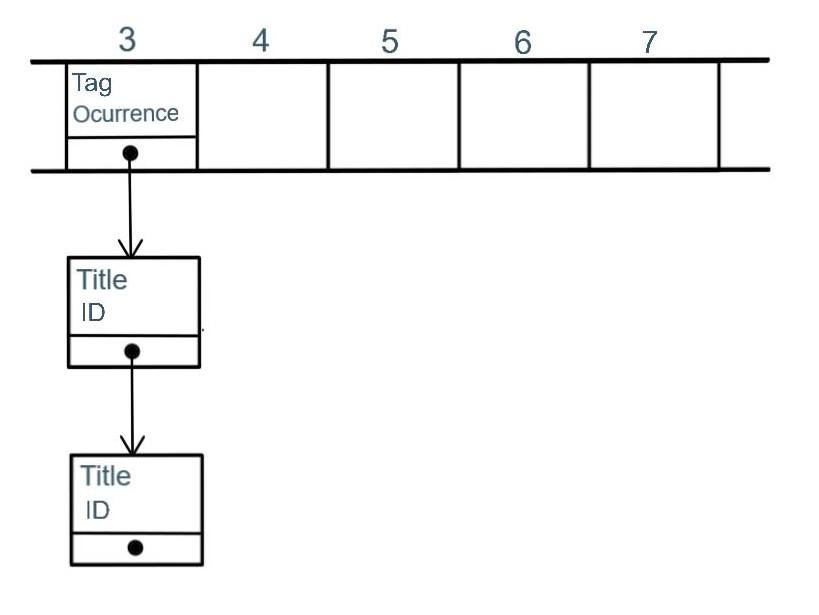
\includegraphics[scale=0.40]{estrutura}
    \caption{\label{fig:controller}Concepção da estrutura de dados}
    \end{figure}
    \newpage
    Para correta inserção na estrutura definimos uma função generate, que é chamada no final de cada notícia, a percorremos o array de tags temporário.
    \begin{verbatim}
    int generate(char *tag, char *tit, char *id, tagList tags ){
        int i = 0;
        int n  = strlen(tag);
        int ntit = strlen(tit);
        int nid  = strlen(id);
    
        Titulo titulo = malloc(sizeof(struct tBucket));
        titulo->titulo = malloc(sizeof(char) * ntit);
        strcpy(titulo->titulo,tit);
        titulo->id = malloc(sizeof(char) * nid);
        strcpy(titulo->id,id);
        titulo->next = NULL;
    
        while( i < MAX && tags[i] != NULL ){
                if(!strcmp(tag,tags[i]->tag)){
                if(tags[i]->titulo){
                    titulo->next = tags[i]->titulo;
                    tags[i]->titulo = titulo;
                }
                else
                    (tags[i]->titulo) = titulo;
                (tags[i]->n)++;
                    break;
                }
                else
                    i++;
        }
    
        if( i < MAX && tags[i] == NULL){
                TAG tmp = malloc(sizeof(struct tagBucket));
                tmp->tag = malloc(sizeof(char) * n);
                strcpy(tmp->tag,tag);
                tmp->n = 1;
                tags[i] = tmp;
            tags[i]->titulo = titulo;
                return 0;
        }
        else
                return 1;
    }
    \end{verbatim}
    \subsection{Main}
    Para tratamento dos dados de input e respectiva apresentação da informação tratada foi desenvolvida a seguinte main:
    \begin{verbatim}
    int main(){
        yylex();
        Titulo tmp;
        FILE *fp;
        fp = fopen("tags.html", "w");
        fprintf(fp, "<head><meta charset=\"UTF-8\"></head>");
        fprintf(fp, "<html><body><h1>Índice de tags</h1>");
        for(int i = 0; i < MAX && ltag[i] != NULL; i++){
            fprintf(fp, "<li>Tag: %s | Ocorrência: %d <p>\n\n", ltag[i]->tag,ltag[i]->n);
            for(tmp = ltag[i]->titulo; tmp; tmp = tmp->next)
                fprintf(fp, "<p>
                <a href=file:///Users/ruiazevedo/Desktop/Universidade/PL/PL/%s>%s</a></p>",
                tmp->id,tmp->titulo);
            fprintf(fp, "</p></li>");
        }
        fprintf(fp, "</body></html>");
        return 0;
    }
    \end{verbatim}
    \section{Apresentação de Resultados}
    Primeiramente, apresentamos um exemplo de uma notícia como input, e o respetivo HTML gerado.

    \subsection{Input}
    \begin{verbatim}
<pub>
#TAG: tag:{Eduardo dos Santos} tag:{Petróleo} tag:{mensagem} tag:{preços} 
#ID:{post-6243 post type-post status-publish format-standard has-post-thumbnail hentry 
category-nacional tag-eduardo-dos-santos tag-petróleo tag-mensagem tag-preços}
Nacional

2015 será um ano dif­ícil, diz o Presidente. Igual aos outros, acrescenta o Povo
PARTILHE VIA:     
#DATE: [116eb] Redação F8 - 29 de Dezembro de 2014
2015 será um ano dif­cil, diz o Presidente. Igual aos outros, acrescenta o Povo - Folha 8

A baixa no preço do barril de petróleo, verificada desde Junho, está a levar o Executivo de Eduardo
dos Santos a tratar estratégias para contornar as dificuldades desencadeadas. Ou seja, com o preço
do petróleo em alta ou em baixa, serão sempre os mais pobres a pagar a factura.

...

Depois de um último ajustamento ao preço dos combust­íveis, em Setembro passado, com um aumento
médio de 25\% ao consumidor no gasóleo e gasolina, na quarta-feira passada, registou-se a um novo
reajustamento de 20\% nos preços dos mesmos tipos de combust­íveis.      

Etiquetas: Eduardo dos SantosPetrleomensagempreos
</pub>
    \end{verbatim}
    \subsection{Output}
    \begin{verbatim}
<html>
<head>
    <meta charset="UTF-8">
    <pub id =post-6243>
    <title>2015 será um ano dif­ícil, diz o Presidente. Igual aos outros, acrescenta o Povo</title>
</head>
<body>
    <h2><author_date>Redação F8 - 29 de Dezembro de 2014</author_date></h2>
    <hr>
    <p>
    <tags>Tags:
        <li><tag>Eduardo dos Santos</tag></li>
        <li><tag>Petróleo</tag></li>
        <li><tag>mensagem</tag></li>
        <li><tag>preços</tag></li>
    </tags>
    </p>
    <hr>
    <p>	<category>Nacional</category></p>
    <hr>
    <text>
A baixa no preço do barril de petróleo, verificada desde Junho, está a levar o Executivo de Eduardo
dos Santos a tratar estratégias para contornar as dificuldades desencadeadas. Ou seja, com o preço
do petróleo em alta ou em baixa, serão sempre os mais pobres a pagar a factura.

...

Depois de um último ajustamento ao preço dos combust­íveis, em Setembro passado, com um aumento
médio de 25% ao consumidor no gasóleo e gasolina, na quarta-feira passada, registou-se a um novo
reajustamento de 20% nos preços dos mesmos tipos de combust­íveis.        
    </text>
</body>
</html>
    \end{verbatim}

    \begin{figure}
    \centering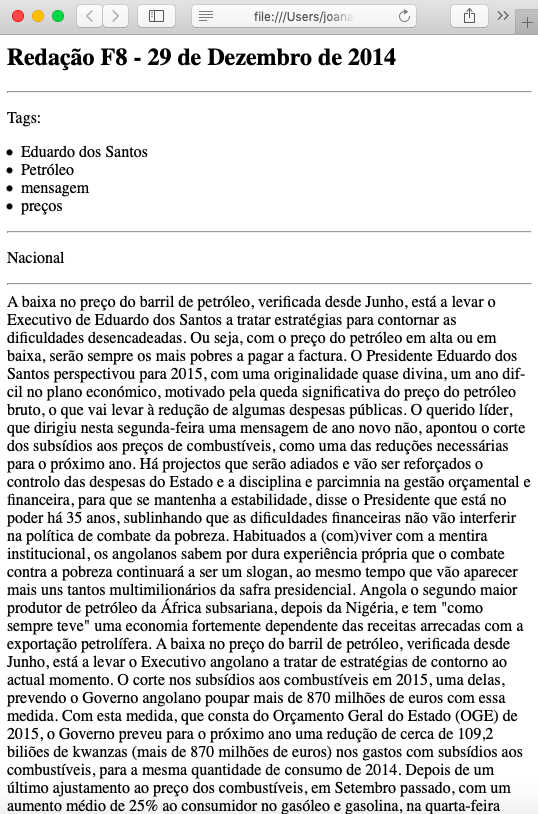
\includegraphics[scale=0.50]{pageHTML}
    \caption{\label{fig:controller}Página HTML da notícia}
    \end{figure}
    \newpage

    \begin{figure}
    \centering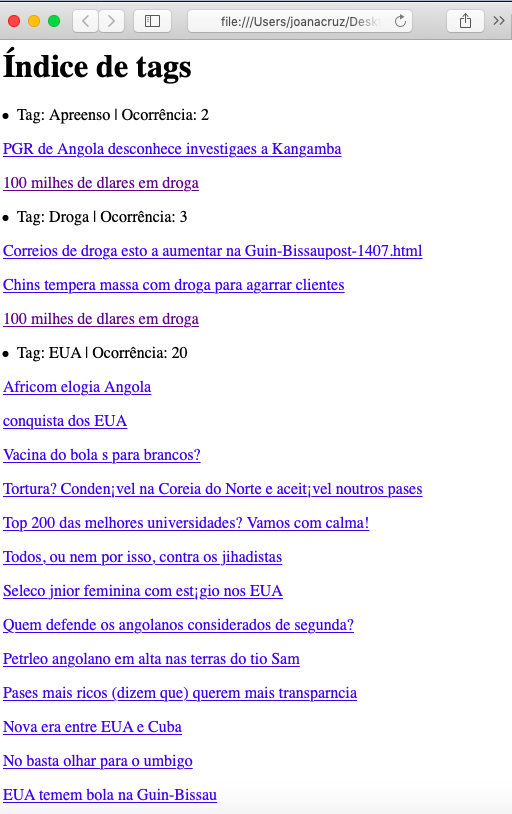
\includegraphics[scale=0.50]{tagsHTML}
    \caption{\label{fig:controller}Página HTML do índice de tags}
    \end{figure}

    \newpage
    \newpage

    \section{Conclusão} 
    Dado os resultados obtidos, podemos concluir que conseguimos estabelecer um conjunto
    de padrões que processam da forma mais precisa possível o ficheiro recebido. No entanto, dado
    os milhares de notícias a processar, poderá haver alguma que não corresponda aos padrões que definimos, o que levaria
    a uma análise ainda mais detalhada à estrutura das notícias para resolver esses problemas específicos.
    Ao identificar os vários elementos que compõem uma notícia foi possível formatar as páginas HTML com a informação
    relevante de uma notícia, isto é, título, tags, identificador, data e conteúdo.
    O FLEX revelou-se uma ferramenta essencial no contexto do processamento de linguagens permitindo filtrar toda a informação
    pretendida de uma maneira simples e eficaz.

    \newpage
    \section{Código FLEX}
    Listagem do código desenvolvido no decorrer do projecto.
    \begin{verbatim}
%{
    #include <string.h>
    #include <stdio.h>
    #include <stdlib.h>
    
    #define MAXTAGPOST 20
    #define MAX 10000
    
    /*  --------------------------  Estruturas  ----------------------------------*/
    
    // Estrutura para guardar o titulo de um artigo e respetivo id
    typedef struct tBucket{
        char *titulo;
        char *id;
        struct tBucket *next;
    }*Titulo;
    
    // Estrutura para guardar as tags, nr de ocorrencias e correspondencia tag -> artigo
    typedef struct tagBucket{
        char *tag;
            int n;
        Titulo titulo;
    }*TAG;
    
    // Lista de todas as tags e respetivos artigos
    typedef TAG tagList[MAX];
    
    // Função que vai gerando a lista de tags e respetivos titulos
    int generate(char *tag, char *tit, char *id, tagList tags ){
            int i = 0;
            int n  = strlen(tag);
        int ntit = strlen(tit);
        int nid  = strlen(id);
    
        Titulo titulo = malloc(sizeof(struct tBucket));
        titulo->titulo = malloc(sizeof(char) * ntit);
        strcpy(titulo->titulo,tit);
        titulo->id = malloc(sizeof(char) * nid);
        strcpy(titulo->id,id);
        titulo->next = NULL;
    
            while( i < MAX && tags[i] != NULL ){
                if(!strcmp(tag,tags[i]->tag)){
                if(tags[i]->titulo){
                    titulo->next = tags[i]->titulo;
                    tags[i]->titulo = titulo;
                }
                else
                    (tags[i]->titulo) = titulo;
                (tags[i]->n)++;
                    break;
                }
                else
                    i++;
            }
    
            if( i < MAX && tags[i] == NULL){
                TAG tmp = malloc(sizeof(struct tagBucket));
                tmp->tag = malloc(sizeof(char) * n);
                strcpy(tmp->tag,tag);
                tmp->n = 1;
                tags[i] = tmp;
            tags[i]->titulo = titulo;
                return 0;
            }
            else
                return 1;
    }
    
    /*  ---------------------------  Variáveis  ----------------------------------*/
    
    tagList ltag;
    char * tagsPost[MAXTAGPOST];
    char * title;
    char * id;
    char * category;
    char * text;
    char * date;
    int numberTags = 0;
    int j = 0;
    
    %}
    
    /*  -------------------------  Start conditions  -----------------------------*/
    
    %x TAGS
    %x TAG
    %x DATE
    %x ID
    %x CLEAN
    %x CATEGORY
    %x TITLE
    %x TEXT
    
    /*  ------------------------------  Flex  ------------------------------------*/
    
    %%
    
    #TAG:   			{BEGIN TAGS; numberTags = 0;}
    <TAGS>tag:\{ 		{BEGIN TAG;}
    <TAGS># 			{BEGIN INITIAL;}
    
    <TAG>\}   			{BEGIN TAGS;}
    <TAG>[^}]+ 			{tagsPost[numberTags++]=strdup(yytext);}
    
    ID:\{				{BEGIN ID;}
    <ID>[^ ]+			{id = strdup(yytext); BEGIN CLEAN;}
    
    <CLEAN>[^}]+\}\n	{BEGIN CATEGORY;}
    
    <CATEGORY>.+\n\n    {yytext[yyleng-2] = '\0'; category = strdup(yytext); BEGIN TITLE;}
    
    <TITLE>.+			{title = strdup(yytext);}
    <TITLE>\n\n      	{BEGIN INITIAL;}
    
    #DATE:\ *\[[^]]+\]\ *   {BEGIN DATE;}
    <DATE>[^\n]+ 		 	{date = strdup(yytext);}
    <DATE>\n[^\n]*\n\n 		{BEGIN TEXT;}
    
    <TEXT>[^<]+			{text = strdup(yytext); BEGIN INITIAL;}
    
    
    \<\/pub\>			{FILE *fp;
                char * idPost = strdup(id);
                char *idP = strcat(idPost,".html");
                fp = fopen(idP, "w");
                fprintf(fp, "<html>\n<head>\n\t<meta charset=\"UTF-8\">
                \n\t<pub id =%s>\n\t<title>%s</title>\n</head>\n", id, title);
                fprintf(fp, "<body>\n\t<h2><author_date>%s</author_date>
                </h2>\n\t<hr>\n\t<p>\n\t<tags>Tags:\n", date);
                for(j= 0; j < numberTags; j++){
                    generate(tagsPost[j], title, idP, ltag);
                    fprintf(fp,"\t\t<li><tag>%s</tag></li>\n", tagsPost[j]);
                }
                fprintf(fp,"\t</tags>\n\t</p>\n\t<hr>\n\t<p>\t<category>%s
                </category></p>\n\t<hr>\n\t<text>\n%s\n\t</text>\n</body>\n</html>", category, text);
                fclose(fp);}
    
    %%
    
    int yywrap(){
        return 1;
    }
    
    /*  ------------------------------  Main  ------------------------------------*/
    
    int main(){
        yylex();
        Titulo tmp;
        FILE *fp;
        fp = fopen("tags.html", "w");
        fprintf(fp, "<head><meta charset=\"UTF-8\"></head>");
        fprintf(fp, "<html><body><h1>Índice de tags</h1>");
    
        for(int i = 0; i < MAX && ltag[i] != NULL; i++){
            fprintf(fp, "\n<li>Tag: %s | Ocorrência: %d <p>\n\n", ltag[i]->tag,ltag[i]->n);
            for(tmp = ltag[i]->titulo; tmp; tmp = tmp->next)
                fprintf(fp, "\n<p>
                e<a href=file:///Users/joanacruz/Desktop/PL/%s>%s</a></p>", tmp->id,tmp->titulo);
            fprintf(fp, "</p></li>");
        }
        fprintf(fp, "</body></html>");
        return 0;
    }
    \end{verbatim}
    
    \end{document}
    